\documentclass[aspectratio=169,11pt]{beamer}
\usetheme{default}
\setbeamertemplate{navigation symbols}{}
\setbeamertemplate{footline}{%
  \hfill\insertframenumber/\inserttotalframenumber\hspace*{4pt}\vspace{2pt}%
}
\usepackage{lmodern}
\usepackage[most]{tcolorbox}
\usepackage{listings}
\usepackage{tikz}
\usetikzlibrary{arrows.meta,positioning,shapes.geometric,fit,backgrounds}
\usepackage{booktabs}
\usepackage{hyperref}

\definecolor{lcgreen}{HTML}{2E7D32}
\definecolor{lcblue}{HTML}{1565C0}
\definecolor{lcorange}{HTML}{EF6C00}
\definecolor{lcred}{HTML}{C62828}
\definecolor{codebg}{HTML}{F5F5F5}
\definecolor{docgray}{gray}{0.55}

\newtcolorbox{conceptbox}[1][]{colback=yellow!20,colframe=yellow!60!black,title=#1,fonttitle=\bfseries}
\newtcolorbox{warningbox}[1][]{colback=red!15,colframe=red!60!black,title=#1,fonttitle=\bfseries}
\newtcolorbox{tipbox}[1][]{colback=green!10,colframe=green!50!black,title=#1,fonttitle=\bfseries}
\newtcolorbox{codebox}[1][]{colback=blue!10,colframe=blue!40!black,title=#1,fonttitle=\bfseries}

\lstset{
  basicstyle=\ttfamily\scriptsize,
  backgroundcolor=\color{codebg},
  breaklines=true,
  frame=single,
  rulecolor=\color{blue!40!black},
  keywordstyle=\color{lcblue}\bfseries,
  stringstyle=\color{lcgreen},
  commentstyle=\color{docgray}\itshape,
  language=Python,
  showstringspaces=false,
  tabsize=2,
  xleftmargin=2pt,
  xrightmargin=2pt,
}

\newcommand{\docref}[1]{{\scriptsize\color{docgray}[Docs: #1]}}

\title{LangChain Section 10}
\subtitle{Callbacks, Streaming \& Tracing}
\author{LangChain v1.2.x (March 2026)}
\date{}

\begin{document}

%============================================================================
% TITLE SLIDE
%============================================================================

\begin{frame}
  \titlepage
  \vspace{-2cm}
  \begin{center}
    {\small Observability, performance monitoring, and real-time event streaming}
  \end{center}
\end{frame}

%============================================================================
% SECTION 1: MENTAL MODEL
%============================================================================

\begin{frame}[fragile]
  \frametitle{Mental Model: Observability as First-Class}

  \begin{center}
    \textbf{Modern LLM apps need visibility into every step}
  \end{center}

  \vspace{0.5cm}

  \begin{itemize}
    \item \textbf{What's happening?} Trace execution flow
    \item \textbf{When is it happening?} Track latency and timing
    \item \textbf{What's it costing?} Monitor token usage
    \item \textbf{Is it working?} Debug failures in production
  \end{itemize}

  \vspace{0.8cm}

  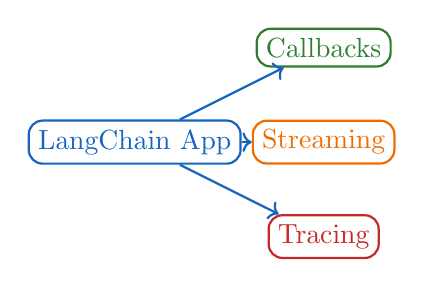
\begin{tikzpicture}[scale=0.8]
    \node[draw, lcblue, thick, rectangle, rounded corners=5pt] (app) at (0,0) {LangChain App};
    \node[draw, lcgreen, thick, rectangle, rounded corners=5pt] (cb) at (3,1.5) {Callbacks};
    \node[draw, lcorange, thick, rectangle, rounded corners=5pt] (stream) at (3,0) {Streaming};
    \node[draw, lcred, thick, rectangle, rounded corners=5pt] (trace) at (3,-1.5) {Tracing};

    \draw[->, lcblue, thick] (app) -- (cb);
    \draw[->, lcblue, thick] (app) -- (stream);
    \draw[->, lcblue, thick] (app) -- (trace);
  \end{tikzpicture}

  \vspace{0.5cm}
  \docref{Observability in LangChain}
\end{frame}

%============================================================================
% SECTION 2: WHY OBSERVABILITY MATTERS
%============================================================================

\begin{frame}
  \frametitle{Why Observability Matters}

  \begin{columns}[T]
    \column{0.48\textwidth}
    \textbf{Development:}
    \begin{itemize}
      \item Debug complex chains
      \item Understand token flow
      \item Identify bottlenecks
      \item Test edge cases
    \end{itemize}

    \column{0.48\textwidth}
    \textbf{Production:}
    \begin{itemize}
      \item Monitor cost/usage
      \item Catch failures early
      \item Improve performance
      \item Audit decisions
    \end{itemize}
  \end{columns}

  \vspace{0.8cm}

  \begin{center}
    \begin{tcolorbox}[colback=lcblue!10, colframe=lcblue, title=Key Insight]
      Without observability, LLM systems become black boxes
    \end{tcolorbox}
  \end{center}

  \vspace{0.5cm}

  LangChain provides three complementary tools:
  \begin{enumerate}
    \item \textbf{Callbacks} — react to events in real-time
    \item \textbf{Streaming} — get results token-by-token
    \item \textbf{Tracing} — capture complete execution history
  \end{enumerate}
\end{frame}

%============================================================================
% SECTION 3: THE CALLBACK SYSTEM
%============================================================================

\begin{frame}[fragile]
  \frametitle{The Callback System: BaseCallbackHandler}

  \begin{conceptbox}[Core Idea]
    Callbacks let you hook into LangChain events and react to them
  \end{conceptbox}

  \vspace{0.5cm}

  \begin{lstlisting}
from langchain_core.callbacks import BaseCallbackHandler

class MyCallback(BaseCallbackHandler):
    """Custom handler for LangChain events."""

    def on_llm_start(self, serialized, inputs, **kwargs):
        print(f"LLM starting with: {inputs}")

    def on_llm_end(self, response, **kwargs):
        print(f"LLM finished: {response}")
  \end{lstlisting}

  \vspace{0.4cm}

  Key methods exist for:
  \begin{itemize}
    \item LLM lifecycle: \texttt{on\_llm\_start}, \texttt{on\_llm\_end}, \texttt{on\_llm\_error}
    \item Tool usage: \texttt{on\_tool\_start}, \texttt{on\_tool\_end}
    \item Chain execution: \texttt{on\_chain\_start}, \texttt{on\_chain\_end}
    \item Token streaming: \texttt{on\_llm\_new\_token}
  \end{itemize}

  \docref{BaseCallbackHandler API}
\end{frame}

%============================================================================
% SECTION 4: BUILT-IN CALLBACK EVENTS
%============================================================================

\begin{frame}
  \frametitle{Built-in Callback Events}

  \begin{table}
    \small
    \centering
    \begin{tabular}{ll}
      \toprule
      \textbf{Event} & \textbf{Triggered When} \\
      \midrule
      \texttt{on\_llm\_start} & LLM call begins \\
      \texttt{on\_llm\_end} & LLM call completes \\
      \texttt{on\_llm\_new\_token} & Token streamed from LLM \\
      \texttt{on\_tool\_start} & Tool invocation begins \\
      \texttt{on\_tool\_end} & Tool invocation completes \\
      \texttt{on\_chain\_start} & Chain/runnable starts \\
      \texttt{on\_chain\_end} & Chain/runnable finishes \\
      \texttt{on\_retriever\_start} & Retriever search begins \\
      \texttt{on\_retriever\_end} & Retriever search completes \\
      \texttt{on\_text} & Text output generated \\
      \bottomrule
    \end{tabular}
  \end{table}

  \vspace{0.5cm}

  \begin{tipbox}[Pro Tip]
    Not all handlers need to implement all methods — implement only what you need
  \end{tipbox}

  \docref{Callback Events Reference}
\end{frame}

%============================================================================
% SECTION 5: CREATING CUSTOM CALLBACK HANDLERS
%============================================================================

\begin{frame}[fragile]
  \frametitle{Creating Custom Callback Handlers}

  \begin{lstlisting}
from langchain_core.callbacks import BaseCallbackHandler
import json

class LoggingCallback(BaseCallbackHandler):
    def on_llm_start(self, serialized, inputs, **kwargs):
        print(f"Model: {serialized.get('name')}")
        print(f"Prompt: {inputs.get('prompts', [])}")

    def on_llm_end(self, response, **kwargs):
        msg = response.generations[0][0].text
        tokens = response.llm_output.get('usage', {})
        print(f"Output: {msg}")
        print(f"Tokens: {json.dumps(tokens)}")

    def on_llm_error(self, error, **kwargs):
        print(f"ERROR: {error}")
  \end{lstlisting}

  \vspace{0.3cm}

  \begin{tipbox}[Async Callbacks]
    For async chains, implement \texttt{on\_llm\_start} (async version exists too)
  \end{tipbox}

  \docref{Custom Callbacks}
\end{frame}

%============================================================================
% SECTION 6: STREAMING TOKENS
%============================================================================

\begin{frame}[fragile]
  \frametitle{Streaming Token-by-Token: stream() \& astream()}

  \begin{lstlisting}
from langchain_openai import ChatOpenAI

llm = ChatOpenAI(model="gpt-4o", streaming=True)

# Synchronous streaming
for chunk in llm.stream("Explain quantum computing"):
    print(chunk.content, end="", flush=True)

# Asynchronous streaming
async def stream_response():
    async for chunk in llm.astream("Explain quantum"):
        print(chunk.content, end="", flush=True)

import asyncio
asyncio.run(stream_response())
  \end{lstlisting}

  \vspace{0.3cm}

  \begin{conceptbox}[When to Use]
    Use \texttt{stream()} for real-time user feedback, \texttt{astream()} for web apps
  \end{conceptbox}

  \docref{Streaming Reference}
\end{frame}

%============================================================================
% SECTION 7: ASTREAM_EVENTS
%============================================================================

\begin{frame}[fragile]
  \frametitle{astream\_events() — Universal Streaming Interface}

  \begin{lstlisting}
from langchain_openai import ChatOpenAI
from langchain_core.callbacks import AsyncIteratorCallbackHandler

llm = ChatOpenAI(model="gpt-4o")

# Stream ALL events from a runnable
async def main():
    async for event in llm.astream_events(
        {"messages": [("human", "Hello")]},
        version="v2"
    ):
        print(f"{event['event']}: {event}")

# Events include:
# - on_llm_start, on_llm_stream, on_llm_end
# - on_chain_start, on_chain_stream, on_chain_end
  \end{lstlisting}

  \vspace{0.3cm}

  \begin{tipbox}[Advantage]
    Single interface handles all runnable types uniformly
  \end{tipbox}

  \docref{astream\_events Documentation}
\end{frame}

%============================================================================
% SECTION 8: EVENT TYPES AND FILTERING
%============================================================================

\begin{frame}[fragile]
  \frametitle{Event Types and How to Filter Them}

  \begin{lstlisting}
async def process_events():
    async for event in llm.astream_events(prompt):
        event_type = event["event"]

        # Filter by type
        if event_type == "on_llm_stream":
            token = event["data"]["chunk"].content
            print(f"Token: {token}")

        elif event_type == "on_chain_end":
            result = event["data"]["output"]
            print(f"Final: {result}")

        # Ignore internal events
        if not event_type.startswith("on_"):
            continue
  \end{lstlisting}

  \vspace{0.3cm}

  Common event structures:
  \begin{itemize}
    \item \texttt{event} — type name (\texttt{"on\_llm\_start"}, etc.)
    \item \texttt{data} — event data (chunks, outputs, errors)
    \item \texttt{run\_id} — trace identifier for correlation
  \end{itemize}

  \docref{Event Structure}
\end{frame}

%============================================================================
% SECTION 9: STREAMING IN WEB APPS
%============================================================================

\begin{frame}[fragile]
  \frametitle{Streaming in Web Apps (FastAPI/SSE)}

  \begin{lstlisting}
from fastapi import FastAPI
from fastapi.responses import StreamingResponse
from langchain_openai import ChatOpenAI

app = FastAPI()
llm = ChatOpenAI(model="gpt-4o")

@app.post("/chat/stream")
async def chat_stream(message: str):
    async def generate():
        async for chunk in llm.astream(message):
            yield f"data: {chunk.content}\n\n"

    return StreamingResponse(
        generate(),
        media_type="text/event-stream"
    )
  \end{lstlisting}

  \vspace{0.3cm}

  Client side (JavaScript):
  \begin{lstlisting}
const es = new EventSource("/chat/stream?message=...");
es.onmessage = (e) => console.log(e.data);
es.onerror = () => es.close();
  \end{lstlisting}

  \docref{FastAPI + Streaming Example}
\end{frame}

%============================================================================
% SECTION 10: LANGSMITH TRACING
%============================================================================

\begin{frame}
  \frametitle{LangSmith Tracing: Automatic Capture}

  \begin{center}
    \textbf{LangSmith is LangChain's observability platform}
  \end{center}

  \vspace{0.5cm}

  \begin{columns}[T]
    \column{0.5\textwidth}
    \textbf{What it captures:}
    \begin{itemize}
      \item Full execution traces
      \item Token usage (prompt + completion)
      \item Latency per step
      \item Inputs and outputs
      \item Errors and exceptions
      \item Custom metadata
    \end{itemize}

    \column{0.5\textwidth}
    \textbf{Features:}
    \begin{itemize}
      \item Web dashboard
      \item Performance analytics
      \item A/B testing
      \item Dataset curation
      \item Debugging tools
    \end{itemize}
  \end{columns}

  \vspace{0.5cm}

  \begin{conceptbox}[Key Point]
    Tracing is automatic — zero code changes needed
  \end{conceptbox}

  \docref{LangSmith Documentation}
\end{frame}

%============================================================================
% SECTION 11: SETTING UP LANGSMITH
%============================================================================

\begin{frame}[fragile]
  \frametitle{Setting Up LangSmith}

  \begin{enumerate}
    \item \textbf{Get API key:} Sign up at \texttt{smith.langchain.com}
    \item \textbf{Set environment variable:}
  \end{enumerate}

  \begin{lstlisting}
# In shell or .env file
export LANGCHAIN_TRACING_V2=true
export LANGCHAIN_API_KEY="ls_..."
export LANGCHAIN_PROJECT="my-project"
  \end{lstlisting}

  \vspace{0.3cm}

  \begin{enumerate}
    \setcounter{enumi}{2}
    \item \textbf{Run your code} — traces appear automatically
  \end{enumerate}

  \begin{lstlisting}
from langchain_openai import ChatOpenAI

llm = ChatOpenAI(model="gpt-4o")
response = llm.invoke("Hello!")
# ^ Automatically traced to LangSmith
  \end{lstlisting}

  \vspace{0.3cm}

  \begin{warningbox}[Important]
    Never commit your API key! Use environment variables
  \end{warningbox}

  \docref{LangSmith Setup}
\end{frame}

%============================================================================
% SECTION 12: READING AND INTERPRETING TRACES
%============================================================================

\begin{frame}
  \frametitle{Reading and Interpreting Traces}

  \begin{center}
    \textbf{LangSmith dashboard shows:}
  \end{center}

  \vspace{0.5cm}

  \begin{columns}[T]
    \column{0.48\textwidth}
    \begin{itemize}
      \item \textbf{Trace graph} — hierarchical execution flow
      \item \textbf{Latency} — time per step (ms)
      \item \textbf{Token count} — input/output tokens
      \item \textbf{Cost} — estimated API cost
    \end{itemize}

    \column{0.48\textwidth}
    \begin{itemize}
      \item \textbf{Inputs/Outputs} — full data logged
      \item \textbf{Errors} — exceptions with stack traces
      \item \textbf{Metadata} — custom tags/context
      \item \textbf{Feedback} — human ratings
    \end{itemize}
  \end{columns}

  \vspace{0.8cm}

  \begin{tipbox}[How to Use]
    Use traces to identify slowdowns, understand token usage, and debug failures
  \end{tipbox}

  \docref{Reading Traces}
\end{frame}

%============================================================================
% SECTION 13: METADATA AND TAGS
%============================================================================

\begin{frame}[fragile]
  \frametitle{Adding Metadata and Tags to Traces}

  \begin{lstlisting}
from langchain_openai import ChatOpenAI
from langchain_core.callbacks import CallbackConfig

llm = ChatOpenAI(model="gpt-4o")

# Add metadata via invoke
response = llm.invoke(
    "Hello",
    config={
        "run_name": "greeting",
        "tags": ["production", "v1.2"],
        "metadata": {
            "user_id": "user_123",
            "session": "abc-def",
            "experiment": "temperature_0.7"
        }
    }
)
  \end{lstlisting}

  \vspace{0.3cm}

  Benefits:
  \begin{itemize}
    \item Filter traces in LangSmith by tags
    \item Correlate with external systems
    \item Track A/B experiments
    \item Organize by user, session, or version
  \end{itemize}

  \docref{Metadata Configuration}
\end{frame}

%============================================================================
% SECTION 14: CUSTOM SPANS WITH @TRACEABLE
%============================================================================

\begin{frame}[fragile]
  \frametitle{Custom Spans with @traceable Decorator}

  \begin{lstlisting}
from langsmith import traceable
from langchain_openai import ChatOpenAI

@traceable
def summarize(text: str) -> str:
    """Custom function traced as a span."""
    llm = ChatOpenAI(model="gpt-4o")
    response = llm.invoke(f"Summarize: {text}")
    return response.content

@traceable
async def process_documents(docs: list) -> list:
    """Async function with tracing."""
    results = []
    for doc in docs:
        summary = summarize(doc)  # Nested trace
        results.append(summary)
    return results

# Use normally - traces captured automatically
result = summarize("Long text here...")
  \end{lstlisting}

  \vspace{0.3cm}

  \begin{tipbox}[Benefit]
    Nest custom functions and see full hierarchy in LangSmith
  \end{tipbox}

  \docref{@traceable Decorator}
\end{frame}

%============================================================================
% SECTION 15: DATA FLOW DIAGRAM
%============================================================================

\begin{frame}
  \frametitle{Callback/Trace Data Flow Architecture}

  \begin{center}
    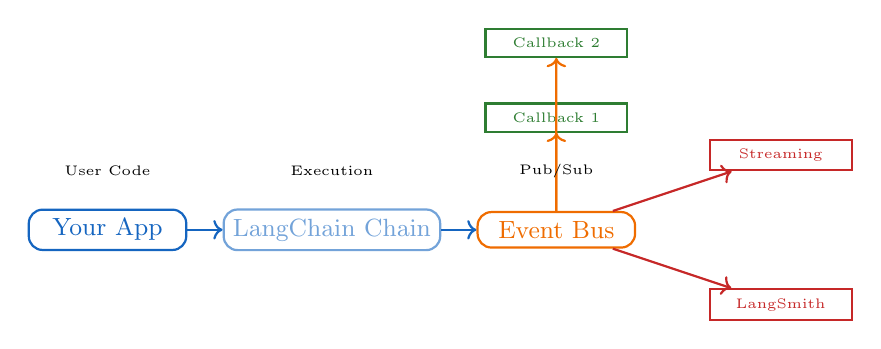
\begin{tikzpicture}[scale=0.95, every node/.style={font=\small}]
      % Main app
      \node[draw, lcblue, thick, minimum width=2cm, rectangle, rounded corners=5pt] (app) at (0,0) {Your App};

      % LangChain chain
      \node[draw, lcblue!60, thick, minimum width=2cm, rectangle, rounded corners=5pt] (chain) at (3,0) {LangChain Chain};

      % Event bus
      \node[draw, lcorange, thick, minimum width=2cm, rectangle, rounded corners=5pt] (events) at (6,0) {Event Bus};

      % Callback handlers
      \node[draw, lcgreen, thick, minimum width=1.8cm] (cb1) at (6,1.5) {\tiny Callback 1};
      \node[draw, lcgreen, thick, minimum width=1.8cm] (cb2) at (6,2.5) {\tiny Callback 2};

      % Streaming
      \node[draw, lcred, thick, minimum width=1.8cm] (stream) at (9,1) {\tiny Streaming};

      % LangSmith
      \node[draw, lcred, thick, minimum width=1.8cm] (smith) at (9,-1) {\tiny LangSmith};

      % Arrows
      \draw[->, lcblue, thick] (app) -- (chain);
      \draw[->, lcblue, thick] (chain) -- (events);
      \draw[->, lcorange, thick] (events) -- (cb1);
      \draw[->, lcorange, thick] (events) -- (cb2);
      \draw[->, lcred, thick] (events) -- (stream);
      \draw[->, lcred, thick] (events) -- (smith);

      % Labels
      \node[above=0.3cm of app, font=\tiny] {User Code};
      \node[above=0.3cm of chain, font=\tiny] {Execution};
      \node[above=0.3cm of events, font=\tiny] {Pub/Sub};
    \end{tikzpicture}
  \end{center}

  \vspace{0.3cm}

  \small All execution flows through the event bus, enabling parallel observability
\end{frame}

%============================================================================
% SECTION 16: PERFORMANCE MONITORING
%============================================================================

\begin{frame}[fragile]
  \frametitle{Performance Monitoring: Latency, Tokens, Cost}

  \begin{lstlisting}
from langchain_openai import ChatOpenAI
import time

class MetricsCallback:
    def on_llm_start(self, **kwargs):
        self.start = time.time()

    def on_llm_end(self, response, **kwargs):
        elapsed = time.time() - self.start
        tokens = response.llm_output.get("usage", {})

        print(f"Latency: {elapsed:.2f}s")
        print(f"Input tokens: {tokens.get('prompt_tokens')}")
        print(f"Output tokens: {tokens.get('completion_tokens')}")

        # Estimate cost (GPT-4o: $0.03/$0.06 per 1M tokens)
        total = tokens.get('prompt_tokens', 0) + \
                tokens.get('completion_tokens', 0)
        cost = total / 1_000_000 * 0.045
        print(f"Est. cost: ${cost:.4f}")
  \end{lstlisting}

  \docref{Performance Monitoring}
\end{frame}

%============================================================================
% SECTION 17: DEBUGGING WITH VERBOSE
%============================================================================

\begin{frame}[fragile]
  \frametitle{Debugging with Verbose Mode and Trace Inspection}

  \begin{lstlisting}
from langchain_openai import ChatOpenAI
from langchain.callbacks import StdOutCallbackHandler

llm = ChatOpenAI(
    model="gpt-4o",
    verbose=True,  # Enable verbose logging
    callbacks=[StdOutCallbackHandler()]
)

response = llm.invoke("Explain neural networks")
# Outputs: Full trace to stdout
  \end{lstlisting}

  \vspace{0.3cm}

  \textbf{Verbose output includes:}
  \begin{itemize}
    \item Prompt sent to LLM
    \item Model response
    \item Token counts
    \item Latency
  \end{itemize}

  \vspace{0.3cm}

  \begin{warningbox}[Caution]
    Verbose mode can be noisy — use selectively in development
  \end{warningbox}

  \docref{Verbose Debugging}
\end{frame}

%============================================================================
% SECTION 18: COMMON PITFALLS
%============================================================================

\begin{frame}[fragile]
  \frametitle{Common Pitfalls and How to Avoid Them}

  \begin{warningbox}[Pitfall 1: Blocking Callbacks]
    Async chains with sync callbacks can cause deadlocks. Use \texttt{async def} in async contexts.
  \end{warningbox}

  \vspace{0.3cm}

  \begin{lstlisting}
# WRONG: Sync callback in async chain
class BadCallback(BaseCallbackHandler):
    def on_llm_end(self, response):
        time.sleep(1)  # Blocks event loop!

# RIGHT: Async callback
class GoodCallback(BaseCallbackHandler):
    async def on_llm_end(self, response):
        await asyncio.sleep(1)  # Non-blocking
  \end{lstlisting}

  \vspace{0.3cm}

  \textbf{Other pitfalls:}
  \begin{itemize}
    \item \textbf{Missing imports} — ensure callbacks in scope
    \item \textbf{Wrong event names} — check case and spelling
    \item \textbf{API key errors} — verify \texttt{LANGCHAIN\_API\_KEY} set
    \item \textbf{Too much logging} — sample events in production
  \end{itemize}

  \docref{Debugging Callbacks}
\end{frame}

%============================================================================
% SECTION 19: SUMMARY & CHEAT SHEET
%============================================================================

\begin{frame}
  \frametitle{Summary: Callbacks, Streaming \& Tracing}

  \textbf{Three Pillars of Observability:}

  \vspace{0.3cm}

  \begin{table}
    \small
    \centering
    \begin{tabular}{p{1.8cm}p{3.5cm}p{2.5cm}}
      \toprule
      \textbf{Tool} & \textbf{Purpose} & \textbf{When} \\
      \midrule
      Callbacks & React to events in real-time & Dev \& prod \\
      Streaming & Get results token-by-token & Web UIs \\
      Tracing & Capture full execution history & Analysis \& debug \\
      \bottomrule
    \end{tabular}
  \end{table}

  \vspace{0.5cm}

  \textbf{Quick Start:}
  \begin{enumerate}
    \item \textbf{Add callbacks:} Extend \texttt{BaseCallbackHandler}
    \item \textbf{Stream results:} Use \texttt{.stream()} or \texttt{.astream()}
    \item \textbf{Enable tracing:} Set env vars (\texttt{LANGCHAIN\_TRACING\_V2})
    \item \textbf{Monitor:} Check LangSmith dashboard
  \end{enumerate}

  \vspace{0.5cm}

  \docref{Section 10 Complete}
\end{frame}

%============================================================================
% SECTION 20: CHEAT SHEET
%============================================================================

\begin{frame}[fragile]
  \frametitle{Quick Reference Cheat Sheet (Part 1)}

  \textbf{Custom Callback:}
  \begin{lstlisting}
from langchain_core.callbacks import BaseCallbackHandler

class MyCallback(BaseCallbackHandler):
    def on_llm_end(self, response, **kw):
        print(response)
  \end{lstlisting}

  \textbf{Streaming:}
  \begin{lstlisting}
for chunk in llm.stream(prompt):
    print(chunk.content)
  \end{lstlisting}

  \textbf{Async Streaming:}
  \begin{lstlisting}
async for chunk in llm.astream(prompt):
    print(chunk.content)
  \end{lstlisting}
\end{frame}

%============================================================================
% SECTION 21: CHEAT SHEET PART 2
%============================================================================

\begin{frame}[fragile]
  \frametitle{Quick Reference Cheat Sheet (Part 2)}

  \textbf{Event Streaming:}
  \begin{lstlisting}
async for event in llm.astream_events(prompt):
    if event["event"] == "on_llm_stream":
        print(event["data"]["chunk"].content)
  \end{lstlisting}

  \textbf{LangSmith Setup:}
  \begin{lstlisting}
export LANGCHAIN_TRACING_V2=true
export LANGCHAIN_API_KEY="ls_..."
# Then run code normally
  \end{lstlisting}

  \textbf{Add Metadata:}
  \begin{lstlisting}
llm.invoke(prompt, config={
    "tags": ["prod"],
    "metadata": {"user": "id"}
})
  \end{lstlisting}
\end{frame}

%============================================================================
% SECTION 22: SELF-CHECK QUESTIONS
%============================================================================

\begin{frame}
  \frametitle{Self-Check: Do You Understand?}

  \begin{enumerate}
    \item What are the three main observability tools in LangChain?
    \vspace{0.3cm}

    \item When would you use callbacks vs. streaming vs. tracing?
    \vspace{0.3cm}

    \item How do you create a custom callback handler?
    \vspace{0.3cm}

    \item What's the difference between \texttt{stream()} and \texttt{astream\_events()}?
    \vspace{0.3cm}

    \item How do you set up LangSmith tracing? (3 steps)
    \vspace{0.3cm}

    \item What's a common pitfall when using callbacks in async chains?
    \vspace{0.3cm}

    \item How can you add custom metadata to traces?
  \end{enumerate}

  \vspace{0.5cm}

  \small \textit{Answers: See previous slides and documentation links}
\end{frame}

%============================================================================
% SECTION 23: KEY TAKEAWAYS
%============================================================================

\begin{frame}
  \frametitle{Key Takeaways}

  \begin{conceptbox}[1. Observability First]
    Build tracing and monitoring into your LLM apps from day one
  \end{conceptbox}

  \vspace{0.4cm}

  \begin{conceptbox}[2. Three Complementary Tools]
    Callbacks for hooks, streaming for UX, tracing for analysis
  \end{conceptbox}

  \vspace{0.4cm}

  \begin{conceptbox}[3. LangSmith = Free Observability]
    Minimal setup for powerful insights — use it!
  \end{conceptbox}

  \vspace{0.4cm}

  \begin{conceptbox}[4. Production Readiness]
    Monitoring, debugging, and cost tracking are non-negotiable
  \end{conceptbox}
\end{frame}

%============================================================================
% SECTION 24: NEXT STEPS
%============================================================================

\begin{frame}
  \frametitle{Next Steps}

  \textbf{Immediate:}
  \begin{enumerate}
    \item Implement a custom callback in your current project
    \item Enable streaming for user-facing features
    \item Sign up for LangSmith and enable tracing
  \end{enumerate}

  \vspace{0.5cm}

  \textbf{Deeper exploration:}
  \begin{itemize}
    \item Build a performance dashboard using callback metrics
    \item Create custom spans for domain-specific logic
    \item Set up alerts based on trace metrics
    \item Use LangSmith datasets for evaluation
  \end{itemize}

  \vspace{0.5cm}

  \textbf{Resources:}
  \begin{itemize}
    \item LangChain callbacks docs
    \item LangSmith platform guide
    \item Example projects in langchain-ai/langchain repo
  \end{itemize}
\end{frame}

%============================================================================
% SECTION 25: Q&A
%============================================================================

\begin{frame}
  \frametitle{Questions?}

  \begin{center}
    \Large
    \vspace{2cm}
    \textbf{LangChain v1.2.x}

    \vspace{0.5cm}

    Section 10: Callbacks, Streaming \& Tracing

    \vspace{2cm}

    \small Covered:
    \begin{itemize}
      \item Callback system and custom handlers
      \item Real-time streaming and events
      \item LangSmith tracing and observability
      \item Performance monitoring and debugging
    \end{itemize}
  \end{center}
\end{frame}

\end{document}
